\section{OO Software Metrics}

\key{Control Flow Graphs}{Cyclomatic Complexity}{CK Metrics}

\defn{Metric}{quantitative measure of degree to which a
system, component or process possesses a given
attribute}

\defn{Indicator}{combination of metrics that provide insight into the
product/process}

\rem{metrics differs from measures in the sense that metrics are functions which
output measures~\cite{metricsWiki}}

\subsubsection{Motivation}

\begin{itemize}
	\item Budgeting 
	\item To create a baseline, in order to compare the impact of new tools
	\item Establish productivity trends and estimate staffing needs
	\item Improve software quality
\end{itemize}

\subsection{How can quality be measured?}

\par{In 1992 , Basili \cite{basili92} suggested a \ita{top-down} goal oriented
framework, to define what could me used as a measurement}

\begin{enumerate}
	\item Develop a set of goals
	\item Develop a set of questions which characterize those goals
	\item Specify the metrics required to answer 2
	\item Develop appropriate mechanisms for data collection and analysis
	\item Collect, validate and analyse the data
	\item Analyse in a \ita{post-mortem} fashion
	\item Provide feedback
\end{enumerate}

\subsubsection{Control Flow Graphs}

\defn{CFG}{a graph representing all possible paths that might be transverses
during the execution of a program} 

\par{We represent blocks of code as nodes in a graph, and draw edges between two
nodes \ita{iff} the execution of one of a node could transfer control to the one
being connected to it}

\par{In order to draw a CFG, we start by breaking the code into its major blocks
by identifying (1) Methods ; (2) Method Blocks ; (3) Decision Points . We then
translate this into nodes and connect them according to all possible execution states}

\ex{
\vphantom{.\\[2mm]}


\begin{minipage}{\linewidth}
      \centering
      \begin{minipage}{0.45\linewidth}
          \begin{figure}[H]
              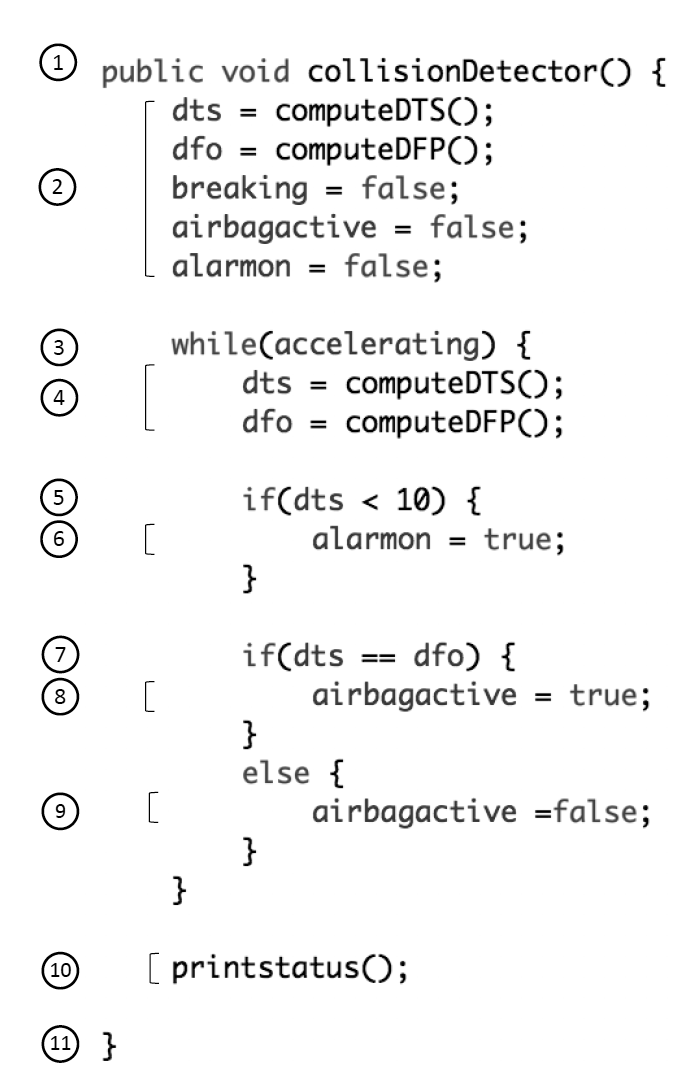
\includegraphics[width=\linewidth]{cfg}
          \end{figure}
      \end{minipage}
      \hspace{0.05\linewidth}
\begin{minipage}{0.45\linewidth}
          \begin{figure}[H]
              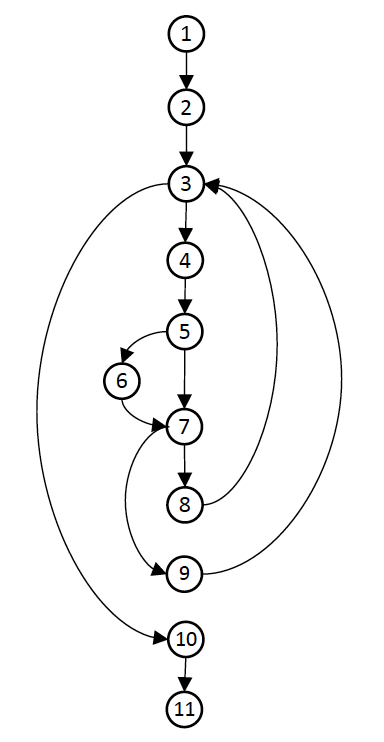
\includegraphics[width=\linewidth]{cfg2}
          \end{figure}
      \end{minipage}
\end{minipage}
}


\defn{Cyclomatic Number $V(G)$}{ of a graph $G$ on $n$ vertices and $e$ edges
with $p$ connected component. $V(G) = e - n + 2p$}

\par{Given the CFG, McCabe~\cite{mccabe76} introduced a graphic-theoretic
complexity measure and showed how it could be used to manage and control program
complexity. The goal was \ita{"to find a mathematical technique that
will provide a  quantitative basis for modularization and allow us to identify
software modules that will be difficult to test or maintain."} As a rule of
thumb, when restructuring code one aims to start with those with higher $V(G)$,
in order to lower their complexity}

\par{\mymarginpar{Pros \& Cons}~This is a fairly easy to compute metric, and
empirical studies have shown good correlation between cyclomatic complexity and
understandability. However, it is the hard to grasp the flow of data, and its
use might not be appropriate for OO programs.}

\subsection{CK Metrics}

\par{More recently, Chidamber and Kemerer \cite{chidamber_kemerer94}, introduced
6 other metrics, which are still in use today, despite the existence of $300+$
new ones}

\begin{enumerate}
	\item\textbf{WMC} : Weighted Methods per Class
	\item\textbf{DIT} : Depth of Inheritance Tree
	\item\textbf{NOC} : Number of Children
	\item\textbf{CBO} : Coupling Between Objects
	\item\textbf{RFC} : Response For a Class
	\item\textbf{LCOM} : Lack of Cohesion of Methods
\end{enumerate}

\par{A summary of the 6 metrics and how they affect complexity , re-usability
and modularity is presented below}

\begin{figure}[H]
	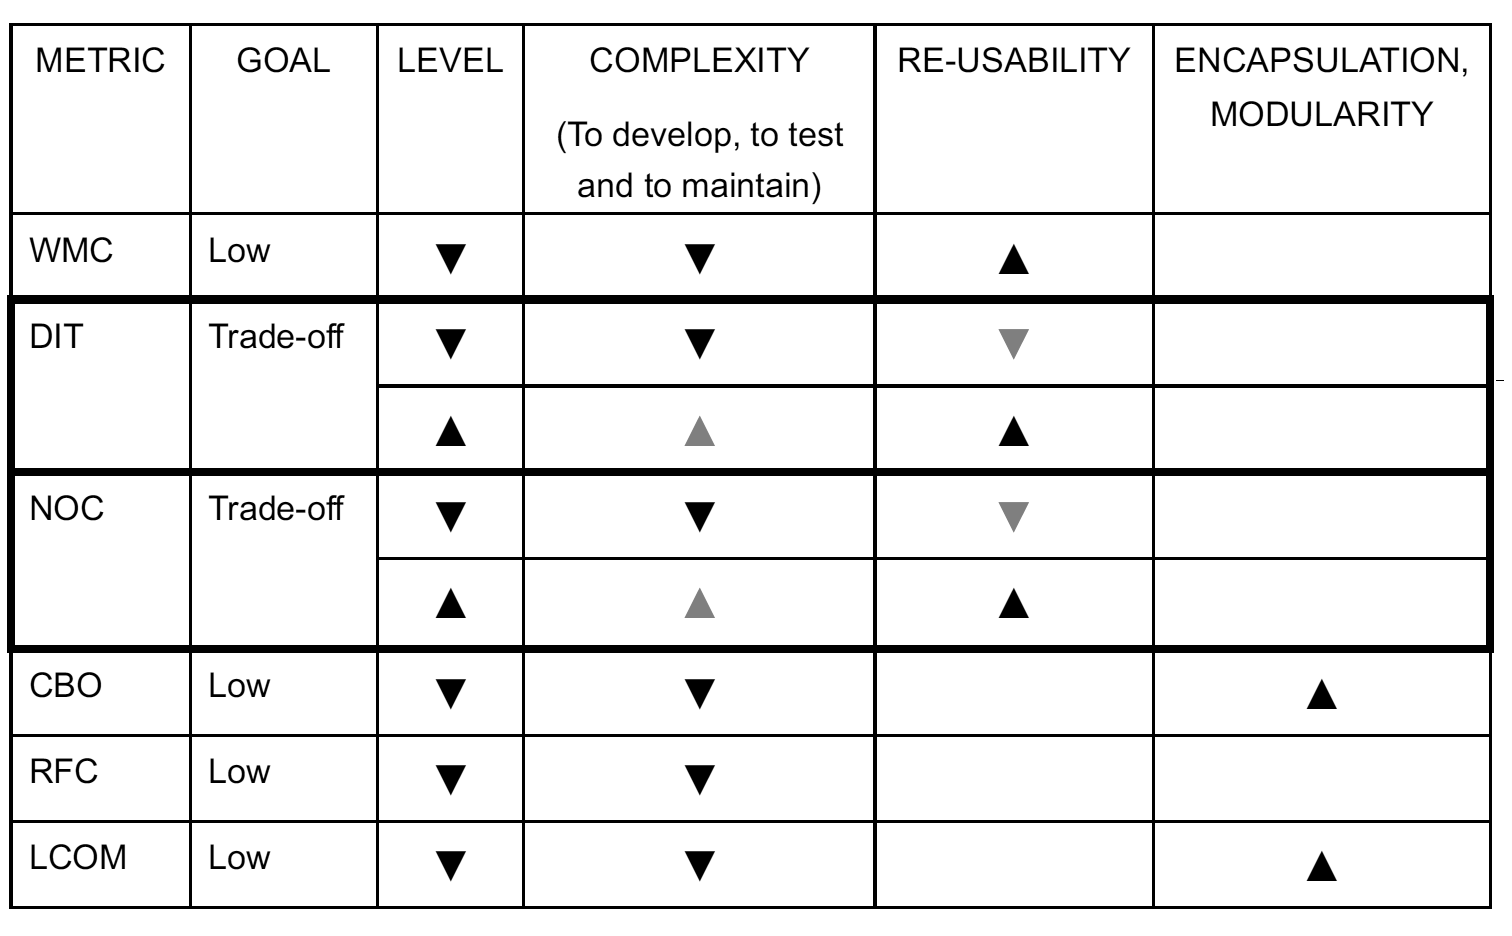
\includegraphics[width=\textwidth]{ck}
	\caption{CK Metrics : Summary}
\end{figure}

\par{Note that there exists a direct relation between the
metric level and complexity level, but sometimes one trades simplicity in favour
of reusability} 

\subsubsection{WMC}

$$\sum_{i=1}^{n}c_i$$

\par{WMC is the sum of the complexities of the methods in a given class, where
$c_i$ represents the McCabe complexity of each method. It acts as a predictor of
how much time and effort is required to develop and maintain that class}

\subsubsection{DIT}

\par{We define DIT as the length of any given node to the root of the tree.
Adding dependent methods, will increase complexity but improve reusability. The
goal is to achieve the appropriate trade-off for a given project}

\subsubsection{NOC}

\par{Similar to DIT, but we look at the number of \ita{direct} children only}

\subsubsection{CBO}

\par{For a given class $C$ , the CBO is the number of other classes to which $C$
is coupled to. Where we define classes to be "coupled" as "operating upon" or
"being operated on"}

\subsubsection{RFC}

\par{The number of methods of a class as well as any other methods being called
by methods within it}

\subsubsection{LCOM}

\par{Counts the sets of methods in a class that are not related
through the sharing of some of the class's fields. It measures the relative
\ita{"tightness"} of a class. The aim is to have as cohesive a class as
possible, otherwise we should wonder if two methods who share little to no
fields should belong to that same class. In practice, the lack of cohesion of a
class is calculated by subtracting the number of method pairs that don't share
access to the same fields by those who do}

\ex{
\vphantom{\\[2mm]}
	\lstinputlisting[language=C]{cohesion.c}
}
